\documentclass[journal,12pt,twocolumn]{IEEEtran}

\usepackage{setspace}
\usepackage{gensymb}
\singlespacing
\usepackage[cmex10]{amsmath}

\usepackage{amsthm}

\usepackage{mathrsfs}
\usepackage{txfonts}
\usepackage{stfloats}
\usepackage{bm}
\usepackage{cite}
\usepackage{cases}
\usepackage{subfig}

\usepackage{longtable}
\usepackage{multirow}

\usepackage{enumitem}
\usepackage{mathtools}
\usepackage{steinmetz}
\usepackage{tikz}
\usepackage{circuitikz}
\usepackage{verbatim}
\usepackage{tfrupee}
\usepackage[breaklinks=true]{hyperref}
\usepackage{graphicx}
\usepackage{tkz-euclide}
\usetikzlibrary{shapes,arrows}

\usetikzlibrary{calc,math}
\usepackage{listings}
    \usepackage{color}                                            %%
    \usepackage{array}                                            %%
    \usepackage{longtable}                                        %%
    \usepackage{calc}                                             %%
    \usepackage{multirow}                                         %%
    \usepackage{hhline}                                           %%
    \usepackage{ifthen}                                           %%
    \usepackage{lscape}     
\usepackage{multicol}
\usepackage{chngcntr}

\DeclareMathOperator*{\Res}{Res}

\renewcommand\thesection{\arabic{section}}
\renewcommand\thesubsection{\thesection.\arabic{subsection}}
\renewcommand\thesubsubsection{\thesubsection.\arabic{subsubsection}}

\renewcommand\thesectiondis{\arabic{section}}
\renewcommand\thesubsectiondis{\thesectiondis.\arabic{subsection}}
\renewcommand\thesubsubsectiondis{\thesubsectiondis.\arabic{subsubsection}}


\hyphenation{op-tical net-works semi-conduc-tor}
\def\inputGnumericTable{}                                 %%

\lstset{
%language=C,
frame=single, 
breaklines=true,
columns=fullflexible
}
\begin{document}


\newtheorem{theorem}{Theorem}[section]
\newtheorem{problem}{Problem}
\newtheorem{proposition}{Proposition}[section]
\newtheorem{lemma}{Lemma}[section]
\newtheorem{corollary}[theorem]{Corollary}
\newtheorem{example}{Example}[section]
\newtheorem{definition}[problem]{Definition}

\newcommand{\BEQA}{\begin{eqnarray}}
\newcommand{\EEQA}{\end{eqnarray}}
\newcommand{\define}{\stackrel{\triangle}{=}}
\bibliographystyle{IEEEtran}
\raggedbottom
\setlength{\parindent}{0pt}
\providecommand{\mbf}{\mathbf}
\providecommand{\pr}[1]{\ensuremath{\Pr\left(#1\right)}}
\providecommand{\qfunc}[1]{\ensuremath{Q\left(#1\right)}}
\providecommand{\sbrak}[1]{\ensuremath{{}\left[#1\right]}}
\providecommand{\lsbrak}[1]{\ensuremath{{}\left[#1\right.}}
\providecommand{\rsbrak}[1]{\ensuremath{{}\left.#1\right]}}
\providecommand{\brak}[1]{\ensuremath{\left(#1\right)}}
\providecommand{\lbrak}[1]{\ensuremath{\left(#1\right.}}
\providecommand{\rbrak}[1]{\ensuremath{\left.#1\right)}}
\providecommand{\cbrak}[1]{\ensuremath{\left\{#1\right\}}}
\providecommand{\lcbrak}[1]{\ensuremath{\left\{#1\right.}}
\providecommand{\rcbrak}[1]{\ensuremath{\left.#1\right\}}}
\theoremstyle{remark}
\newtheorem{rem}{Remark}
\newcommand{\sgn}{\mathop{\mathrm{sgn}}}
\providecommand{\abs}[1]{\left\vert#1\right\vert}
\providecommand{\res}[1]{\Res\displaylimits_{#1}} 
\providecommand{\norm}[1]{\left\lVert#1\right\rVert}
%\providecommand{\norm}[1]{\lVert#1\rVert}
\providecommand{\mtx}[1]{\mathbf{#1}}
\providecommand{\mean}[1]{E\left[ #1 \right]}
\providecommand{\fourier}{\overset{\mathcal{F}}{ \rightleftharpoons}}
%\providecommand{\hilbert}{\overset{\mathcal{H}}{ \rightleftharpoons}}
\providecommand{\system}{\overset{\mathcal{H}}{ \longleftrightarrow}}
	%\newcommand{\solution}[2]{\textbf{Solution:}{#1}}
\newcommand{\solution}{\noindent \textbf{Solution: }}
\newcommand{\cosec}{\,\text{cosec}\,}
\providecommand{\dec}[2]{\ensuremath{\overset{#1}{\underset{#2}{\gtrless}}}}
\newcommand{\myvec}[1]{\ensuremath{\begin{pmatrix}#1\end{pmatrix}}}
\newcommand{\mydet}[1]{\ensuremath{\begin{vmatrix}#1\end{vmatrix}}}
\numberwithin{equation}{subsection}

\makeatletter
\@addtoreset{figure}{problem}
\makeatother
\let\StandardTheFigure\thefigure
\let\vec\mathbf

\renewcommand{\thefigure}{\theproblem}

\def\putbox#1#2#3{\makebox[0in][l]{\makebox[#1][l]{}\raisebox{\baselineskip}[0in][0in]{\raisebox{#2}[0in][0in]{#3}}}}
     \def\rightbox#1{\makebox[0in][r]{#1}}
     \def\centbox#1{\makebox[0in]{#1}}
     \def\topbox#1{\raisebox{-\baselineskip}[0in][0in]{#1}}
     \def\midbox#1{\raisebox{-0.5\baselineskip}[0in][0in]{#1}}
\vspace{3cm}
\title{EE4013 Assignment-1}
\author{Krishna Srikar Durbha - EE18BTECH11014}
\maketitle
\newpage
\bigskip
\renewcommand{\thefigure}{\theenumi}
\renewcommand{\thetable}{\theenumi}
Download all codes from 
\begin{lstlisting}
https://github.com/dks2000dks/IIT-Hyderabad-Semester-Courses/tree/master/EE4013/Assignment1/codes
\end{lstlisting}
%
and latex-tikz codes from 
%
\begin{lstlisting}
https://github.com/dks2000dks/IIT-Hyderabad-Semester-Courses/tree/master/EE4013/Assignment1
\end{lstlisting}
\section{Problem}
Consider the following ANSI C function:
\begin{lstlisting}[language=C]
int SomeFunction(int x, int y){
	if ((x == 1) || (y == 1)) return 1;
	if (x == y) return x;
	if (x > y) return SomeFunction(x-y, y);
	if (x < y) return SomeFunction(x, y-x);
}
\end{lstlisting}
The value of returned by SomeFunction(15,255) is \rule{1cm}{0.15mm}
\section{Solution}
\subsection{Answer}
\quad Let \textbf{SomeFunction} be represented as $f$. The recursion goes as follows:
\[
\begin{split}
&f(15,255) = f(15,240) = f(15,225) = f(15,210)\\
&= f(15,195) = f(15,180) = f(15,165) = f(15,150)\\
&= f(15,135) = f(15,120) = f(15,105) = f(15,90)\\
&= f(15,75) = f(15,60) = f(15,45) = f(15,30)\\
&= f(15,15) = 1
\end{split}\]

\quad One other approach is that knowing or recognising that $f$ is an implementation of Euclidean Algorithm by Subtraction for calculating GCD of positive integers $x$ and $y$.
\begin{align}
	gcd(15,255) = 15 \text{ (As $15 \times 17 = 255$)} 
\end{align}

\subsection{Euclidean Algorithm by Subtraction}
Euclidean Algorithm is a recursive method of finding Greatest Common Divisor of 2 numbers. For some positive integers $a$ and $b$, Euclidean Algorithm by Subtraction repeatedly subtracts the smaller number from the larger one. $gcd(a,b) = gcd(a-b,b)$ considering that $a > b$. We repeat the procedure till convergence i.e both numbers are equal. At this point, the value of either term is the greatest common divisor of our inputs.\\
\textbf{Proof:}\\
Proof involves proving that, subtracting between $a$ and $b$ doesn't change GCD. Let $a$, $b$ be 2 positive integers such that $gcd(a,b) = m$ and $a > b$. So, it can be written as,
\begin{align}
    a = a_{1} \times m \\
    b = b_{1} \times m \\
    gcd(a,b) = m \implies gcd(a_{1}, b_{1}) = 1
\end{align}
We need to prove that $gcd(a-b,b) = m$. We will prove it by contradiction. Let $gcd(a-b,b) = M$ where $M > m \implies 
 k \neq 1$
\begin{align}
    a-b = (a_{1} - b_{1}) \times m\\
    b =  b_{1} \times m\\
    gcd(a-b,b) = M\\
    M = k \times m \text{ (For some integer $k$)}\\
    a-b \equiv 0\ (\textrm{mod}\ M) \text{ and } b \equiv 0\ (\textrm{mod}\ M)\\
    a-b \equiv 0\ (\textrm{mod}\ km) \text{ and } b \equiv 0\ (\textrm{mod}\ km)\\
    a_{1} - b_{1} \equiv 0\ (\textrm{mod}\ k) \text{ and } b_{1} \equiv 0\ (\textrm{mod}\ k)\\
    a_{1} \equiv 0\ (\textrm{mod}\ k) \text{ and } b_{1} \equiv 0\ (\textrm{mod}\ k)
\end{align}
We know that $gcd(a_{1}, b_{1}) = 1$, so $a$ and $b$ cannot have a common divisor $k$. Hence by contradiction, there doesn't exist a $M \neq m$ such that $gcd(a-b, b) = M$. Hence it can be proved that, $gcd(a, b) = gcd(a-b, b) = m$ for $a > b$.\\

\subsubsection{Complexity Analysis}
Let $a > b$ and $T(n)$ denote time complexity of $gcd(a,b)$ where $n = a+b$. Then,
\begin{align}
T(n) = 1 + T(n-b)\\
T(n-b) = 1 + T(n-2b) \text{ if $a > 2b$}\\
T(n-b) = 1 + T(n-a-b) \text{ if $b < a < 2b$}
\end{align}

On assuming $n > (x_{1}a + x_{2}b)$ for some $x_{1}, x_{2}$, $T(n)$ can be written as:
\begin{align}
T(n) = k + T(n - x_{1}a - x_{2}b) \text{ (For $k = x_{1} + x_{2}$)}
\end{align}
No.of steps vary linearly with $n=a+b$. So, in the worst-case scenerio the algorithm performs $a+b$ subtractions. Hence Worst Case Time-Complexity for calculating GCD of $a$ and  $b$ using Euclidean Algorithm by Subtraction is $\mathcal{O}(a + b)$.\\

\begin{figure}[h!]
	\begin{center}
		\resizebox{\columnwidth/1}{!}{% Define block styles
\tikzstyle{dblock} = [diamond, draw, text width=4em, text badly centered, inner sep=0pt, minimum height=2.5em]
\tikzstyle{rblock} = [rectangle, draw, text width=2em, text centered, inner sep=0pt, minimum height=1.5em, rounded corners]
\tikzstyle{eblock} = [ellipse, draw, text width=4em, text centered, inner sep=0pt, minimum height=2.5em]
    
\tikzstyle{line} = [draw, -latex']

\begin{tikzpicture}[node distance = 7.5em, auto]
    % Place nodes
	\node (enter) [eblock] {$a, b$};
    \node (start) [eblock, below of=enter, yshift=2em] {$x=a$ \\ $y=b$};
	\node (condition1) [dblock, below of=start] {$x=1$ \\ or \\ $y=1$};
	\node (return1) [rblock, right of=condition1] {$1$};
	\node (condition2) [dblock, below of=condition1] {$x=y$};
	\node (return2) [rblock, right of=condition2] {$x$};
	\node (condition3) [dblock, below of=condition2] {$x > y$};
	\node (modify1) [eblock, left of=condition3, xshift=-0.75em] {$a = x-y$ \\ $ b = y$};
	\node (condition4) [dblock, below of=condition3] {$x < y$};
	\node (modify2) [eblock, right of=condition4, xshift=3em] {$a = x$ \\ $b = y-x$};
    % Draw edges
	\path [line] (enter) -- (start);
	\path [line] (start) -- (condition1);
	\path [line] (condition1) -- (condition2);
	\path [line] (condition2) -- (condition3);
	\path [line] (condition3) -- (condition4);
	\path [line] (condition1) -- (return1);
	\path [line] (condition2) -- (return2);
	\path [line] (condition3) -- (modify1);
	\path [line] (modify1) |- (enter);
	\path [line] (condition4) -- (modify2);	
	\path [line] (modify2) |- (enter);
\end{tikzpicture}
}
	\end{center}
	\caption{Flowchart of Euclidean Algorithm by Subtraction}
	\label{fig:Input}
\end{figure}

Codes of Euclidean Algorithm by Subtraction:
\begin{lstlisting}
codes/Euclid_Subtraction.py
codes/Euclid_Subtraction.c
\end{lstlisting}

\subsection{Euclidean Algorithm by Division}
Euclidean Algorithm by Division involves divison rather than subtraction. For some positive integers $a$ and $b$, $gcd(a, b) = gcd(b, a \textrm{ mod}\ b)$. We repeat the procedure until convergence.\\

Let $a$ and $b$ be 2 positive integers such that $a > b$. By applying Euclid's Algorithm from $0^{th}$-step,\\
\begin{align}
	a = q_{0}b + r_{0}\label{eq:ED1}\\
	b = q_{1}r_{0} + r_{1}\\
	r_{0} = q_{2}r_{1} + r_{2}\\
	r_{1} = q_{3}r_{2} + r_{3}...
\end{align}
Here $a > b$, $ b > r_{0}$, $r_{0} > r_{1}$, $r_{1} > r_{2}$.. and so on. So, remainders are decreasing after each step.

Let at $n^{th}$-step $r_{n-2} = q_{n}r_{n-1}$ i.e $r_{n} = 0$.
 \begin{align}
    r_{n-2} = q_{n}r_{n-1}\label{eq:ED2}\\
    r_{n-3} = q_{n-1}r_{n-2} + r_{n-1}\\
    r_{n-1} \text{ divides } r_{n-2}, r_{n-3}, r_{n-4},..., r_{1}, r_{0}, b, a\\
    a \equiv 0\ (\textrm{mod}\ r_{n-1}) \text{ and } b \equiv 0\ (\textrm{mod}\ r_{n-1})
\end{align}
So, $r_{n-1}$ is a common divisor of both $a$ and $b$. Let $gcd(a,b) = M \implies M > r_{n-1}$,\\
\begin{align}
    a = a_{1} \times M \text{ and } b = b_{1} \times M\\
    r_{0} = a - q_{0}b = M(a_{1} - q_{0}b_{1})\\
    r_{1} = b - q_{1}r_{0} = M(b_{1} - q_{1}a_{1} + q_{1}q_{0}b_{1})
\end{align}
So, M divides $a, b, r_{0}, r_{1}, ... $ and so on all the following remainders. So, $M$ should divide $r_{n-1}$, which implies $r_{n-1} \geq M$ which is a contraction as $M > r_{n-1}$. Hence by contradiction, there doesn't exist a $M > r_{n-1}$ which is a divisor of $a$ and $b$. So, $gcd(a,b) = r_{n-1}$.\\

\quad On using Euclidean Algorithm by Division the recursion goes as follows:
\[
\begin{split}
&gcd(15,255) = gcd(255,15) = gcd(15,0) = 15
\end{split}\]

\subsubsection{Complexity Analysis}
Let $f_{n}$ denote elements in Pingala Sequence starting from $n=0$ where $f_{0} = 0, f_{1} = 1, f_{2} = 1,...$ and so on. Elements of the sequence can be written as follows:
\begin{align*}
f_{n+2} = 1 \times f_{n+1} + f_{n}\\
f_{n+1} = 1 \times f_{n} + f_{n-1}\\
...........................\\
f_{4} = 1 \times f_{3} + f_{2}\\
f_{3} = 2 \times f_{2}
\end{align*}
The above equations are similar to equations in Euclidean Algorithm by Division i.e from \eqref{eq:ED1} to \eqref{eq:ED2}. Hence it can be proved that $gcd(f_{n+2}, f_{n+1}) = f_{2} = 1$ and takes $n$ steps to converge.\\

If $gcd(a,b)$ takes $n$ steps to converge by using Euclidean Algorithm by Division, then $a \geq f_{n+2}$ and $b \geq f_{n+1}$.\\

\textbf{Proof by Mathematical Induction:}\\
Let $a = 2$ and $b = 1$. Then, $gcd(2,1) = 1$ takes $1$ step to converge. $a \geq f_{3} = 2$ and $b \geq f_{2} = 1$. Assuming statements hold true at ${n-1}^{th}$ step, $gcd(b,a\%b)$ takes $n-1$ steps to converge.
\begin{align}
b \geq f_{n+1}\\
a\%b \geq f_{n}\\
a = q_{0}b + a\%b\\
a \geq b + a\%b\\
a \geq f_{n+1} + f_{n}\\
a \geq f_{n+2}
\end{align}
Hence proved.\\

Let $gcd(a,b)$ takes $n$ steps to converge. Then,
\begin{align}
a \geq f_{n+2}\\
b \geq f_{n+1}\\
f_{n}=\frac{1}{\sqrt{5}}\left(\left(\frac{1+\sqrt{5}}{2}\right)^{n}-\left(\frac{1-\sqrt{5}}{2}\right)^{n}\right)\\
\phi = \frac{1+\sqrt{5}}{2}\\
f_{n} \approx \phi^{n}\\
b \approx \phi^{n+1}\\
n \approx \log_{\phi}{\left(min(a,b)\right)}
\end{align}
So, in the worst-case scenerio the algorithm performs $n \approx \log_{\phi}{\left(min(a,b)\right)} $ divisons. Hence, Worst Case Time-Complexity for calculating GCD of $a$ and  $b$ using Euclidean Algorithm by Division is $\mathcal{O}(\log min(a,b))$.\\

\begin{figure}[h!]
	\begin{center}
		\resizebox{\columnwidth/1}{!}{% Define block styles
\tikzstyle{dblock} = [diamond, draw, text width=4em, text badly centered, inner sep=0pt, minimum height=2.5em]
\tikzstyle{rblock} = [rectangle, draw, text width=2em, text centered, inner sep=0pt, minimum height=1.5em, rounded corners]
\tikzstyle{eblock} = [ellipse, draw, text width=4em, text centered, inner sep=0pt, minimum height=2.5em]
    
\tikzstyle{line} = [draw, -latex']

\begin{tikzpicture}[node distance = 7.5em, auto]
    % Place nodes
	\node (enter) [eblock] {$a, b$};
    \node (start) [eblock, below of=enter, yshift=2em] {$x=a$ \\ $y=b$};
	\node (condition1) [dblock, below of=start, yshift=1em] {$x=0$};
	\node (return1) [rblock, right of=condition1] {$y$};
	\node (condition2) [dblock, below of=condition2, yshift=8em] {$y=0$};
	\node (return2) [rblock, right of=condition2] {$x$};
	\node (condition3) [dblock, below of=condition2] {$x = y$};
	\node (return3) [rblock, right of=condition3] {$x$};
	\node (condition4) [dblock, below of=condition3] {$x > y$};
	\node (modify1) [eblock, left of=condition4, xshift=-0.75em] {$a = y$ \\ $ b = x\%y$};
	\node (condition5) [dblock, below of=condition4] {$x < y$};
	\node (modify2) [eblock, right of=condition5, xshift=3em] {$a = x$ \\ $b = y\%x$};
    % Draw edges
	\path [line] (enter) -- (start);
	\path [line] (start) -- (condition1);
	\path [line] (condition1) -- (condition2);
	\path [line] (condition2) -- (condition3);
	\path [line] (condition3) -- (condition4);
	\path [line] (condition4) -- (condition5);
	\path [line] (condition1) -- (return1);
	\path [line] (condition2) -- (return2);
	\path [line] (condition3) -- (return3);
	\path [line] (condition4) -- (modify1);
	\path [line] (modify1) |- (enter);
	\path [line] (condition5) -- (modify2);	
	\path [line] (modify2) |- (enter);
\end{tikzpicture}
}
	\end{center}
	\caption{Flowchart of Euclidean Algorithm by Division}
	\label{fig:Input}
\end{figure}

Codes of Euclidean Algorithm by Division:
\begin{lstlisting}
codes/Euclid_Division.py
codes/Euclid_Division.c
\end{lstlisting}

\subsection{Comparison between Algorithms:}
The following example illustrates the difference in no.of steps between Euclidean Algorithm by Subtraction and Euclidean Algorithm by Divison. To find GCD of two numbers $24$ and $92$.\\

By Euclid's Subtraction,
\[
\begin{split}
&f(24,92) = f(24,68) = f(24,44) = f(24,20)\\
&= f(4,20) = f(4,16) = f(4,12) = f(4,8)\\
&= f(4,4) = 4
\end{split}\]

By Euclid's Division,
\[
\begin{split}
&f(24,92) = f(92,24) = f(24,20) = f(20,4)\\
&= f(4,0) = 4
\end{split}\]

\begin{table}[!ht]
	\centering
	%%%%%%%%%%%%%%%%%%%%%%%%%%%%%%%%%%%%%%%%%%%%%%%%%%%%%%%%%%%%%%%%%%%%%%
%%                                                                  %%
%%  This is the header of a LaTeX2e file exported from Gnumeric.    %%
%%                                                                  %%
%%  This file can be compiled as it stands or included in another   %%
%%  LaTeX document. The table is based on the longtable package so  %%
%%  the longtable options (headers, footers...) can be set in the   %%
%%  preamble section below (see PRAMBLE).                           %%
%%                                                                  %%
%%  To include the file in another, the following two lines must be %%
%%  in the including file:                                          %%
%%        \def\inputGnumericTable{}                                 %%
%%  at the beginning of the file and:                               %%
%%        \input{name-of-this-file.tex}                             %%
%%  where the table is to be placed. Note also that the including   %%
%%  file must use the following packages for the table to be        %%
%%  rendered correctly:                                             %%
%%    \usepackage[latin1]{inputenc}                                 %%
%%    \usepackage{color}                                            %%
%%    \usepackage{array}                                            %%
%%    \usepackage{longtable}                                        %%
%%    \usepackage{calc}                                             %%
%%    \usepackage{multirow}                                         %%
%%    \usepackage{hhline}                                           %%
%%    \usepackage{ifthen}                                           %%
%%  optionally (for landscape tables embedded in another document): %%
%%    \usepackage{lscape}                                           %%
%%                                                                  %%
%%%%%%%%%%%%%%%%%%%%%%%%%%%%%%%%%%%%%%%%%%%%%%%%%%%%%%%%%%%%%%%%%%%%%%



%%  This section checks if we are begin input into another file or  %%
%%  the file will be compiled alone. First use a macro taken from   %%
%%  the TeXbook ex 7.7 (suggestion of Han-Wen Nienhuys).            %%
\def\ifundefined#1{\expandafter\ifx\csname#1\endcsname\relax}


%%  Check for the \def token for inputed files. If it is not        %%
%%  defined, the file will be processed as a standalone and the     %%
%%  preamble will be used.                                          %%
\ifundefined{inputGnumericTable}

%%  We must be able to close or not the document at the end.        %%
	\def\gnumericTableEnd{\end{document}}


%%%%%%%%%%%%%%%%%%%%%%%%%%%%%%%%%%%%%%%%%%%%%%%%%%%%%%%%%%%%%%%%%%%%%%
%%                                                                  %%
%%  This is the PREAMBLE. Change these values to get the right      %%
%%  paper size and other niceties.                                  %%
%%                                                                  %%
%%%%%%%%%%%%%%%%%%%%%%%%%%%%%%%%%%%%%%%%%%%%%%%%%%%%%%%%%%%%%%%%%%%%%%

	\documentclass[12pt%
			  %,landscape%
                    ]{report}
       \usepackage[latin1]{inputenc}
       \usepackage{fullpage}
       \usepackage{color}
       \usepackage{array}
       \usepackage{longtable}
       \usepackage{calc}
       \usepackage{multirow}
       \usepackage{hhline}
       \usepackage{ifthen}

	\begin{document}


%%  End of the preamble for the standalone. The next section is for %%
%%  documents which are included into other LaTeX2e files.          %%
\else

%%  We are not a stand alone document. For a regular table, we will %%
%%  have no preamble and only define the closing to mean nothing.   %%
    \def\gnumericTableEnd{}

%%  If we want landscape mode in an embedded document, comment out  %%
%%  the line above and uncomment the two below. The table will      %%
%%  begin on a new page and run in landscape mode.                  %%
%       \def\gnumericTableEnd{\end{landscape}}
%       \begin{landscape}


%%  End of the else clause for this file being \input.              %%
\fi

%%%%%%%%%%%%%%%%%%%%%%%%%%%%%%%%%%%%%%%%%%%%%%%%%%%%%%%%%%%%%%%%%%%%%%
%%                                                                  %%
%%  The rest is the gnumeric table, except for the closing          %%
%%  statement. Changes below will alter the table's appearance.     %%
%%                                                                  %%
%%%%%%%%%%%%%%%%%%%%%%%%%%%%%%%%%%%%%%%%%%%%%%%%%%%%%%%%%%%%%%%%%%%%%%

\providecommand{\gnumericmathit}[1]{#1} 
%%  Uncomment the next line if you would like your numbers to be in %%
%%  italics if they are italizised in the gnumeric table.           %%
%\renewcommand{\gnumericmathit}[1]{\mathit{#1}}
\providecommand{\gnumericPB}[1]%
{\let\gnumericTemp=\\#1\let\\=\gnumericTemp\hspace{0pt}}
 \ifundefined{gnumericTableWidthDefined}
        \newlength{\gnumericTableWidth}
        \newlength{\gnumericTableWidthComplete}
        \newlength{\gnumericMultiRowLength}
        \global\def\gnumericTableWidthDefined{}
 \fi
%% The following setting protects this code from babel shorthands.  %%
 \ifthenelse{\isundefined{\languageshorthands}}{}{\languageshorthands{english}}
%%  The default table format retains the relative column widths of  %%
%%  gnumeric. They can easily be changed to c, r or l. In that case %%
%%  you may want to comment out the next line and uncomment the one %%
%%  thereafter                                                      %%
\providecommand\gnumbox{\makebox[0pt]}
%%\providecommand\gnumbox[1][]{\makebox}

%% to adjust positions in multirow situations                       %%
\setlength{\bigstrutjot}{\jot}
\setlength{\extrarowheight}{\doublerulesep}

%%  The \setlongtables command keeps column widths the same across  %%
%%  pages. Simply comment out next line for varying column widths.  %%
\setlongtables

\setlength\gnumericTableWidth{%
	50pt+%
	50pt+%
0pt}
\def\gumericNumCols{5}
\setlength\gnumericTableWidthComplete{\gnumericTableWidth+%
         \tabcolsep*\gumericNumCols*2+\arrayrulewidth*\gumericNumCols}
\ifthenelse{\lengthtest{\gnumericTableWidthComplete > \linewidth}}%
         {\def\gnumericScale{\ratio{\linewidth-%
                        \tabcolsep*\gumericNumCols*2-%
                        \arrayrulewidth*\gumericNumCols}%
{\gnumericTableWidth}}}%
{\def\gnumericScale{1}}

%%%%%%%%%%%%%%%%%%%%%%%%%%%%%%%%%%%%%%%%%%%%%%%%%%%%%%%%%%%%%%%%%%%%%%
%%                                                                  %%
%% The following are the widths of the various columns. We are      %%
%% defining them here because then they are easier to change.       %%
%% Depending on the cell formats we may use them more than once.    %%
%%                                                                  %%
%%%%%%%%%%%%%%%%%%%%%%%%%%%%%%%%%%%%%%%%%%%%%%%%%%%%%%%%%%%%%%%%%%%%%%

\ifthenelse{\isundefined{\gnumericColA}}{\newlength{\gnumericColA}}{}\settowidth{\gnumericColA}{\begin{tabular}{@{}p{45pt*\gnumericScale}@{}}x\end{tabular}}
\ifthenelse{\isundefined{\gnumericColB}}{\newlength{\gnumericColB}}{}\settowidth{\gnumericColB}{\begin{tabular}{@{}p{30pt*\gnumericScale}@{}}x\end{tabular}}
\ifthenelse{\isundefined{\gnumericColC}}{\newlength{\gnumericColC}}{}\settowidth{\gnumericColC}{\begin{tabular}{@{}p{35pt*\gnumericScale}@{}}x\end{tabular}}
\ifthenelse{\isundefined{\gnumericColD}}{\newlength{\gnumericColD}}{}\settowidth{\gnumericColD}{\begin{tabular}{@{}p{30pt*\gnumericScale}@{}}x\end{tabular}}
\ifthenelse{\isundefined{\gnumericColE}}{\newlength{\gnumericColE}}{}\settowidth{\gnumericColE}{\begin{tabular}{@{}p{35pt*\gnumericScale}@{}}x\end{tabular}}

\begin{tabular}[c]{%
	b{\gnumericColA}%
	b{\gnumericColB}%
	b{\gnumericColC}%
	b{\gnumericColD}%
	b{\gnumericColE}%
	}

%%%%%%%%%%%%%%%%%%%%%%%%%%%%%%%%%%%%%%%%%%%%%%%%%%%%%%%%%%%%%%%%%%%%%%
%%  The longtable options. (Caption, headers... see Goosens, p.124) %%
%	\caption{The Table Caption.}             \\	%
% \hline	% Across the top of the table.
%%  The rest of these options are table rows which are placed on    %%
%%  the first, last or every page. Use \multicolumn if you want.    %%

%%  Header for the first page.                                      %%
%	\multicolumn{3}{c}{The First Header} \\ \hline 
%	\multicolumn{1}{c}{colTag}	%Column 1
%	&\multicolumn{1}{c}{colTag}	%Column 2
%	&\multicolumn{1}{c}{colTag}	\\ \hline %Last column
%	\endfirsthead

%%  The running header definition.                                  %%
%	\hline
%	\multicolumn{3}{l}{\ldots\small\slshape continued} \\ \hline
%	\multicolumn{1}{c}{colTag}	%Column 1
%	&\multicolumn{1}{c}{colTag}	%Column 2
%	&\multicolumn{1}{c}{colTag}	\\ \hline %Last column
%	\endhead

%%  The running footer definition.                                  %%
%	\hline
%	\multicolumn{3}{r}{\small\slshape continued\ldots} \\
%	\endfoot

%%  The ending footer definition.                                   %%
%	\multicolumn{3}{c}{That's all folks} \\ \hline 
%	\endlastfoot
%%%%%%%%%%%%%%%%%%%%%%%%%%%%%%%%%%%%%%%%%%%%%%%%%%%%%%%%%%%%%%%%%%%%%%

\hhline{|-|-|-|-|-}
	 \multicolumn{1}{|p{\gnumericColA}|}%
	{\gnumericPB{\centering}$a,b$}
	&\multicolumn{1}{p{\gnumericColB}|}%
	{\gnumericPB{\centering}$N_{-}$}
	&\multicolumn{1}{p{\gnumericColC}|}%
	{\gnumericPB{\centering}$T_{-}(\mu s)$}
	&\multicolumn{1}{p{\gnumericColD}|}%
	{\gnumericPB{\centering}$N_{\%}$}
	&\multicolumn{1}{p{\gnumericColE}|}%
	{\gnumericPB{\centering}$T_{\%}(\mu s)$}
	
\\
\hhline{|-----|}
\hhline{|-----|}
	 \multicolumn{1}{|p{\gnumericColA}|}%
	{\gnumericPB{\centering}$319,50$}
	&\multicolumn{1}{p{\gnumericColB}|}%
	{\gnumericPB{\centering}$14$}
	&\multicolumn{1}{p{\gnumericColC}|}%
	{\gnumericPB{\centering}$14.781$}
	&\multicolumn{1}{p{\gnumericColD}|}%
	{\gnumericPB{\centering}$8$}
	&\multicolumn{1}{p{\gnumericColE}|}%
	{\gnumericPB{\centering}$8.821$}
\\
\hhline{|-----|}
	 \multicolumn{1}{|p{\gnumericColA}|}%
	{\gnumericPB{\centering}$453,369$}
	&\multicolumn{1}{p{\gnumericColB}|}%
	{\gnumericPB{\centering}$14$}
	&\multicolumn{1}{p{\gnumericColC}|}%
	{\gnumericPB{\centering}$15.974$}
	&\multicolumn{1}{p{\gnumericColD}|}%
	{\gnumericPB{\centering}$7$}
	&\multicolumn{1}{p{\gnumericColE}|}%
	{\gnumericPB{\centering}$8.106$}
\\
\hhline{|-----|}
	 \multicolumn{1}{|p{\gnumericColA}|}%
	{\gnumericPB{\centering}$263,810$}
	&\multicolumn{1}{p{\gnumericColB}|}%
	{\gnumericPB{\centering}$18$}
	&\multicolumn{1}{p{\gnumericColC}|}%
	{\gnumericPB{\centering}$18.596$}
	&\multicolumn{1}{p{\gnumericColD}|}%
	{\gnumericPB{\centering}$6$}
	&\multicolumn{1}{p{\gnumericColE}|}%
	{\gnumericPB{\centering}$6.675$}
\\
\hhline{|-----|}
	 \multicolumn{1}{|p{\gnumericColA}|}%
	{\gnumericPB{\centering}$243,929$}
	&\multicolumn{1}{p{\gnumericColB}|}%
	{\gnumericPB{\centering}$18$}
	&\multicolumn{1}{p{\gnumericColC}|}%
	{\gnumericPB{\centering}$19.550$}
	&\multicolumn{1}{p{\gnumericColD}|}%
	{\gnumericPB{\centering}$9$}
	&\multicolumn{1}{p{\gnumericColE}|}%
	{\gnumericPB{\centering}$9.775$}
\\
\hhline{|-----|}
	 \multicolumn{1}{|p{\gnumericColA}|}%
	{\gnumericPB{\centering}$508,609$}
	&\multicolumn{1}{p{\gnumericColB}|}%
	{\gnumericPB{\centering}$41$}
	&\multicolumn{1}{p{\gnumericColC}|}%
	{\gnumericPB{\centering}$56.505$}
	&\multicolumn{1}{p{\gnumericColD}|}%
	{\gnumericPB{\centering}$6$}
	&\multicolumn{1}{p{\gnumericColE}|}%
	{\gnumericPB{\centering}$8.583$}
\\
\hhline{|-|-|-|-|-}
\end{tabular}

\ifthenelse{\isundefined{\languageshorthands}}{}{\languageshorthands{\languagename}}
\gnumericTableEnd

	\caption{Comparison between Euclidean Algorithm by Division and Euclidean Algorithm by Subtraction}
	\label{table:table1}
\end{table}

The difference in no.of steps indicates the performance improvement of Euclidean Algorithm by Division over Euclidean Algorithm by Subtraction.\\

\begin{figure}[!ht]
	\centering
	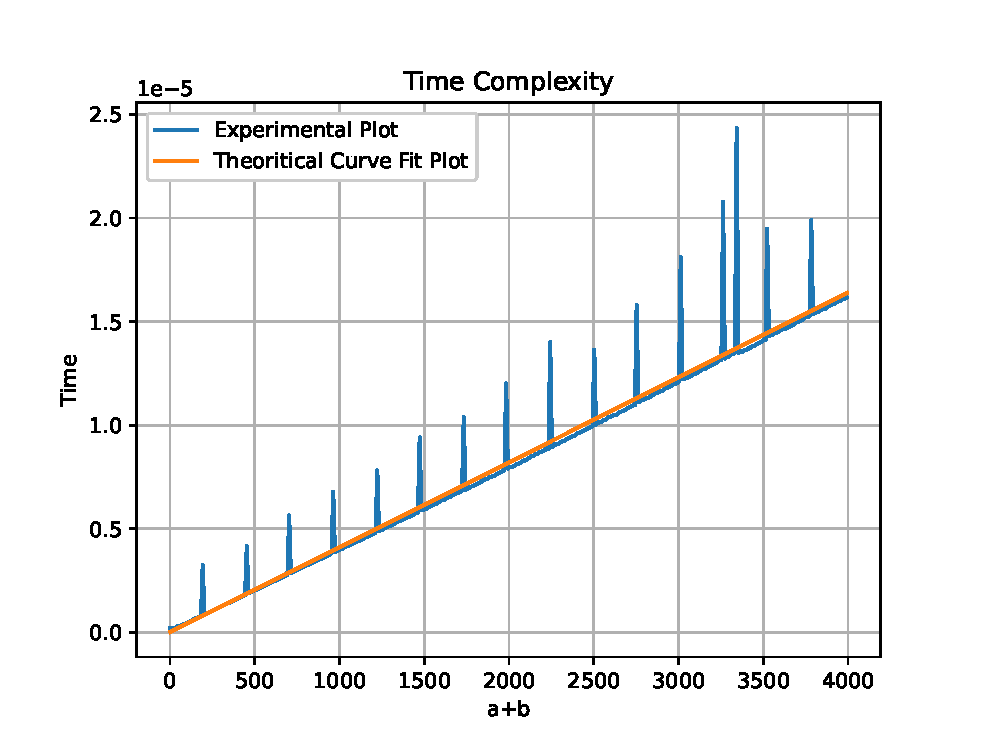
\includegraphics[width=\columnwidth]{figs/Euclid_Subtraction.eps}
	\caption{Plot of Worst-Case Time Complexity of Euclidean Algorithm by Subtraction}
	\label{fig:0}
\end{figure}

\begin{figure}[!ht]
	\centering
	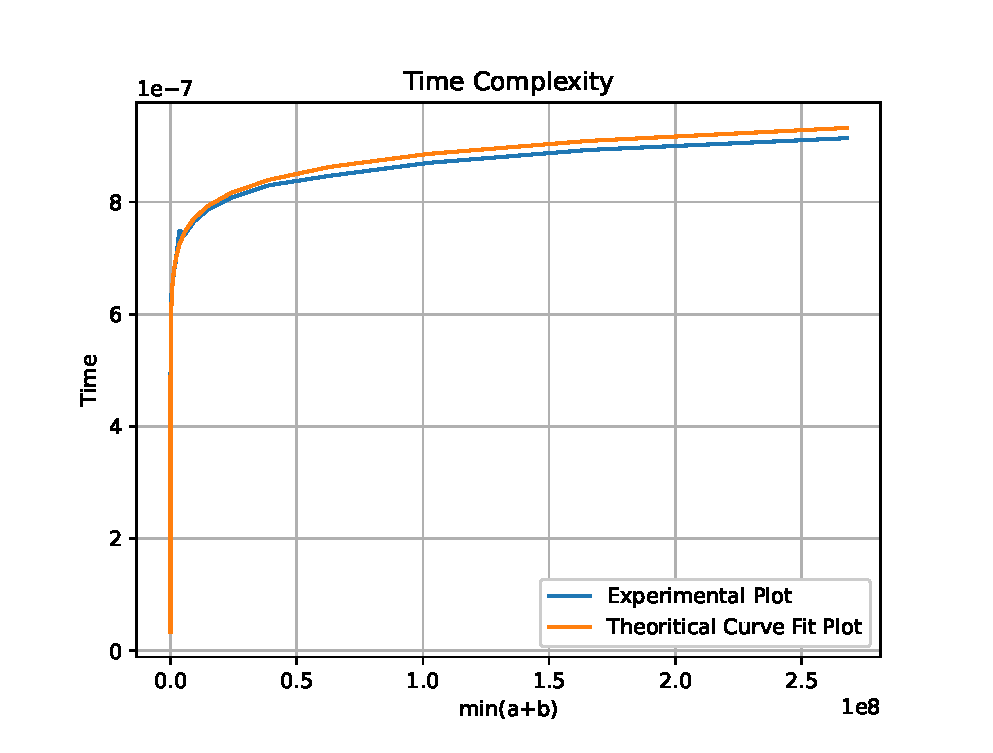
\includegraphics[width=\columnwidth]{figs/Euclid_Division.eps}
	\caption{Plot of Worst-Case Time Complexity of Euclidean Algorithm by Division}
	\label{fig:1}
\end{figure}
\end{document}
